\documentclass{article}[18pt]
\usepackage[utf8]{inputenc}
\usepackage[margin=0.7in]{geometry}
\usepackage{parselines} 
\usepackage{amsmath}
\usepackage{titlesec}
\usepackage{pgfplots}
\usepackage{graphicx}
\usepackage[english]{babel}
\usepackage{fancyhdr}
\usepackage{gensymb}
\usepackage{tikz}
\usetikzlibrary{positioning,scopes,decorations.text}
\pgfplotsset{width=10cm,compat=1.9}

\titlespacing\section{0pt}{14pt plus 4pt minus 2pt}{0pt plus 2pt minus 2pt}
\newlength\tindent
\setlength{\tindent}{\parindent}
\setlength{\parindent}{0pt}
\renewcommand{\indent}{\hspace*{\tindent}}

\pagestyle{fancy}
\fancyhf{}
\rhead{Sam Robbins 13SE}
\lhead{A Level Maths - M2}
\rfoot{Page \thepage}


\begin{document}
\begin{center}
\underline{\huge Dynamics}
\end{center}
\newpage
\begin{center}
\underline{\huge Dynamics Example - F=ma on a slope}
\end{center}
\textit{A car of mass 1500 kg is moving up a straight road, which is inclined at an angle $\theta$ to the
horizontal, where $\sin\theta=\frac{1}{14}$ The resistance to the motion of the car from non-gravitational
forces is constant and is modelled as a single constant force of magnitude 650 N. The car’s
engine is working at a rate of 30 kW.\\
Find the acceleration of the car at the instant when its speed is 15$\text{ms}^{-1}$. }
\\
\\
\textbf{Draw a diagram to represent the question}
\\
\\
\def\iangle{35} % Angle of the inclined plane

\def\down{-90}
\def\arcr{0.5cm} % Radius of the arc used to indicate angles
\begin{tikzpicture}[
    force/.style={>=latex,draw=blue,fill=blue},
    calculatedforce/.style={>=latex,draw=red,fill=red},
    axis/.style={densely dashed,gray,font=\small},
    M/.style={rectangle,draw,fill=lightgray,minimum size=0.5cm,thin},
    m/.style={rectangle,draw=black,fill=lightgray,minimum size=0.3cm,thin},
    plane/.style={draw=black,fill=blue!10},
    string/.style={draw=red, thick},
    pulley/.style={thick},
    scale=2.25
]



    %% Free body diagram of M
    \begin{scope}[rotate=\iangle]
        \node[M,transform shape] (M) {};
        % Draw axes and help lines

        {[axis,-]
            \draw (M.center) -- (0,-1) node[right] {};

            % Indicate angle. The code is a bit awkward.

            \draw[solid,shorten >=0.5pt] (\down-\iangle:\arcr)
                arc(\down-\iangle:\down:\arcr);
            \node at (\down-0.5*\iangle:1.3*\arcr) {$\theta$};
        }

        % Forces
        {[force,->]
            % Assuming that Mg = 1. The normal force will therefore be cos(alpha)
            \draw (M.south) -- ++(0,{cos(\iangle)*1.5}) node[above right] {$R$};
            \draw (M.west) -- ++(-1,0) node[left] {$650N$};
            \draw (M.east) -- ++(1,0) node[above] {$T$};
        
            }
        {[calculatedforce,->]       
        
        \draw (0,-1) -- ++(-0.7,0) node[pos=0,right,sloped] {};
        }
        \draw[black, thick] (-3,-0.25) -- (2,-0.25);
		\node at (0,-1.13) (nodeA) {};
		\node at (-0.7,-1.13) (nodeB) {};
		\draw [decoration={text along path,text={{$1500g\sin\theta$}{}},text align={center}},decorate]  (nodeB) -- (nodeA);



    \end{scope}
    % Draw gravity force. The code is put outside the rotated
    % scope for simplicity. No need to do any angle calculations. 
    \draw[force,->] (M.center) -- ++(0,-1.5) node[below] {$1500g$};
    \draw[black, thick] (-2.31,-1.93) -- (1.76,-1.93);
    \draw[thick, -] (-1.8,-1.93) arc (0:36:0.5);
    \node[] at (-1.93,-1.8) {$\theta$};


    %%



\\
;
\end{tikzpicture}
\\
\\
\textbf{Apply Newton's Second Law (F=ma)}\\
\\
$T-650-1500g\sin\theta=1500a$\\
\\
\textbf{Use $\text{Power=Force}\times\text{Velocity}$}\\
\\
$30,000=T\times15$\\
\\
$T=\dfrac{30,000}{15}=2000$\\
\\
\textbf{Solve, substituting power result into Newton's Second Law result}\\
\\
$2000-650-1500\times9.8\times\frac{1}{14}=1500a$\\
\\
\\
$a=\dfrac{2000-650-1500\times9.8\times\frac{1}{14}}{1500}=0.2$
\newpage
\begin{center}
\underline{\huge Dynamics Example - Momentum and Impulse}
\end{center}

\textit{A ball of mass 0.5 kg is moving with velocity $(10\mathbf{i} + 24\mathbf{j}) \ \text{ms}^{-1}$ when it is struck by a bat.\\
Immediately after the impact the ball is moving with velocity $20\mathbf{i} \ \text{ms}^{-1}$. }
\\
\\
\textit{Find the magnitude of the impulse of the bat on the ball}\\
\\
\textbf{Apply the impulse formula}\\
\\
\textcolor{red}{$I=m(v-u)$}\\
\\
$I=0.5(20\mathbf{i}-(10\mathbf{i}+24\mathbf{j}))=\underline{5\mathbf{i}-12\mathbf{j}}$\\
\\
\textbf{Find the magnitude}\\
\\
$I=\sqrt{5^2+(-12)^2}=\underline{13Ns}$\\
\\
\textit{Find the size of the angle between the vector i and the impulse exerted by the bat on the ball}\\
\\
\\
\textbf{Draw diagram to show vector}\\
\\
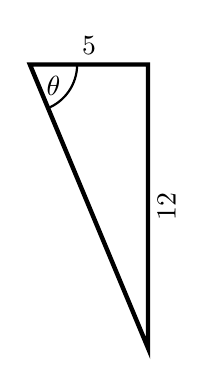
\begin{tikzpicture}[scale=0.3]
\draw[black, ultra thick] (0,0) -- (5,0) -- (5,-12) -- cycle;
\draw (0,0) -- (5,0) node [midway, above, sloped] (TextNode) {$5$};
\draw (5,-12) -- (5,0) node [midway, below, sloped] (TextNode) {$12$};
\draw[thick, -] (2,0) arc (0:-69:2);
\node[] at (1,-0.9) {$\theta$};
\end{tikzpicture}\\
\\
\textbf{Use trigonometry to find angle}\\
\\
$\theta=\arctan\Big(\dfrac{12}{5}\Big)=67.4\degree$\\
\\
\textit{Find the kinetic energy lost by the ball in the impact}\\
\\
\textcolor{red}{$\Delta E_k=E_{k2}-E_{k1}$}\\
\\
$\Delta E_k=\frac{1}{2}\times0.5\times20^2-\frac{1}{2}\times0.5\times(10^2+24^2)=-69J$


\end{document}